\documentclass[12pt]{article}

\usepackage[margin=1in]{geometry}
\usepackage{amsmath, amsthm}
\usepackage{amssymb}
\usepackage{graphicx}
\usepackage{times}
% \usepackage{subcaption}
\usepackage[colorlinks=true, linkcolor=black, citecolor=black, urlcolor=black]{hyperref}


\title{CSCI 5352: Homework 2}
\author{
    Zachary Caterer$^{1,2,3}$ \\
    \small $^1$Department of Computer Science, University of Colorado Boulder \\
    \small $^2$Department of Chemical and Biological Engineering, University of Colorado Boulder \\
    \small $^3$Interdisciplinary Quantitative Biology Program, University of Colorado Boulder
}
\date{\today}

\begin{document}

\maketitle

\subsection*{Collaborators}
I worked with the following people on this assignment:

\begin{itemize}
    \item Ben Braun
    \item Logan Barrios
    \item Luis Paez
    \item Michael Luzadder
    \item Pedro Lemos
\end{itemize}

\section*{Problem 1}

Let \( S_A \) and \( S_B \) be the two subnetworks in the given graph, with \( A \) and \( B \) serving as the only connection between them.

Closeness centrality for a node \( i \) is given by:

\[
C_i = \frac{1}{\ell_i}, \quad \text{where} \quad \ell_i = \frac{1}{n} \sum_{j \neq i} d(i,j)
\]

Thus, the average shortest path lengths for \( A \) and \( B \) are:

\[
\ell_A = \frac{1}{n} \left( \sum_{i \in A} d_A(i) + \sum_{j \in B} d_A(j) + n_B \right)
\]

\[
\ell_B = \frac{1}{n} \left( \sum_{i \in B} d_B(i) + \sum_{j \in A} d_B(j) + n_A \right)
\]

Taking their difference:

\[
\ell_A - \ell_B = \frac{1}{n} (n_B - n_A)
\]

Since \( C_A = \frac{1}{\ell_A} \) and \( C_B = \frac{1}{\ell_B} \), we get:

\[
\frac{1}{C_A} - \frac{1}{C_B} = \frac{1}{n} (n_B - n_A)
\]

Rearranging:

\[
\frac{1}{C_A} + \frac{n_A}{n} = \frac{1}{C_B} + \frac{n_B}{n}
\]


\begin{flushright}
    \( \blacksquare \)
\end{flushright}


\section*{Problem 2}    

\subsection*{Part A}
\begin{enumerate}
    \item Selection Criteria:
    \begin{itemize}
        \item Randomly select two directed edges \( (u,v) \) and \( (x,y) \) from the network.
        \item Since it is a directed network, the order of the nodes in the edge matters. Thus, the two edges are distinct.
    \end{itemize}
    \item The only output configurations that maintains the node $k^{in}$ and $k^{out}$ values are:
    \begin{itemize}
        \item \( (u, x)\) and \( (v, y) \)
    \end{itemize}
    \item Checkes needed on $G'$:
    \begin{itemize}
        \item Ensure no self loops.
        \item Ensure no multiple edges.
        \item Verify the $k^{in}$ and $k^{out}$ values of the nodes remain unchanged.
    \end{itemize}
\end{enumerate}

\subsection*{Part B}
\begin{enumerate}
    \item Selection Criteria:
    \begin{itemize}
        \item Randomly select two directed edges one from each partition, for simplicity sake lets say nodes \( u \) and \( v \) are from partition \( A \) and nodes \( x \) and \( y \) are from partition \( B \). So the two edges are \( (u,x) \) and \( (v,y) \).
    \end{itemize}
    \item Possible output configurations:
    \begin{itemize}
        \item The only option: \( (u, y)\) and \( (v, x) \)
    \end{itemize}
    \item Checkes needed on $G'$:   
    \begin{itemize}
        \item Ensure no self loops.
        \item Ensure no multiple edges.
        \item Ensure $u \neq x$ and $v \neq y$.
        \item Verify the degrees of the nodes remain unchanged.
        \item Veriy the new edges maintain bipartite structure.
    \end{itemize}
\end{enumerate}


\section*{Problem 3}

\textbf{\textit{Need to fix, complete, and check this section.}}\\

Comment on how ``random” Berkeley’s social network was to begin with, in what ways, and
on the rate at which randomization destroys the empirical patterns

\begin{figure}[h]
    \centering
    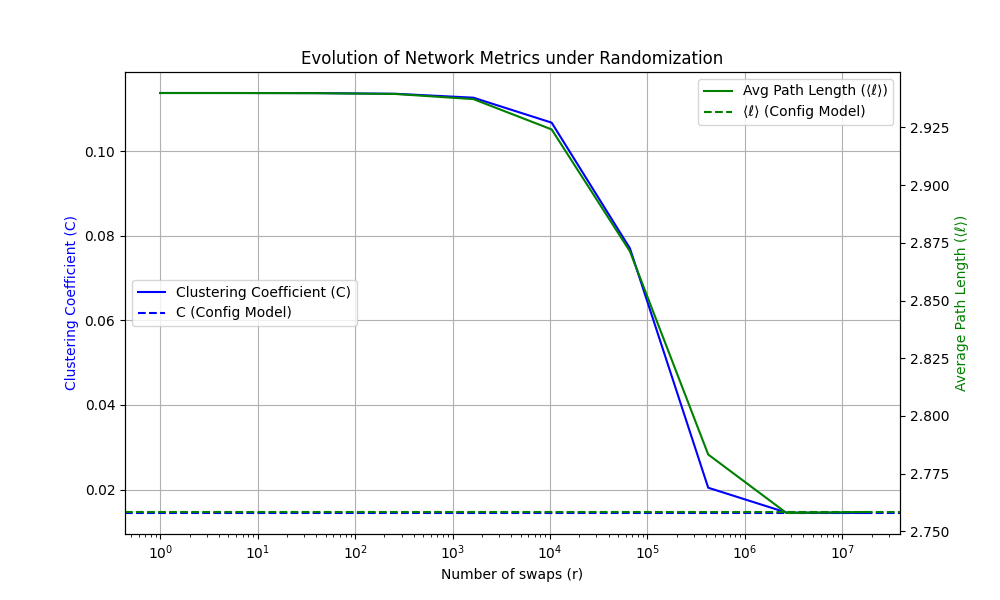
\includegraphics[width=0.8\textwidth]{../figures/network_evolution.png}
    \caption{Evolution of Network Metrics under Randomization. The network metrics are shown as the number of swaps (r/m) increases the Clustering Coefficient (C) and average path length ($\langle \ell \rangle$) of the network decreases. Additionally, the Configuration model for clustering coefficient and average path length are shown in the dashed line.}
    \label{fig:network_evolution}
\end{figure}

\section*{Problem 4}

\subsection*{Social Network -- Moreno Zebra's}
\begin{figure}[h]
    \centering
    \begin{minipage}{0.45\textwidth}
        \centering
        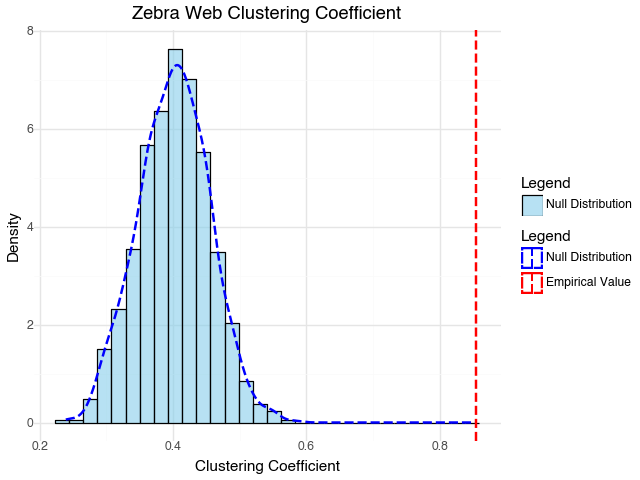
\includegraphics[width=\textwidth]{../figures/zebra_clustering.png}
        % \caption{Moreno Zebra's Social Network}
        \label{fig:zebra_network_clustering}
    \end{minipage}
    \hfill
    \begin{minipage}{0.45\textwidth}
        \centering
        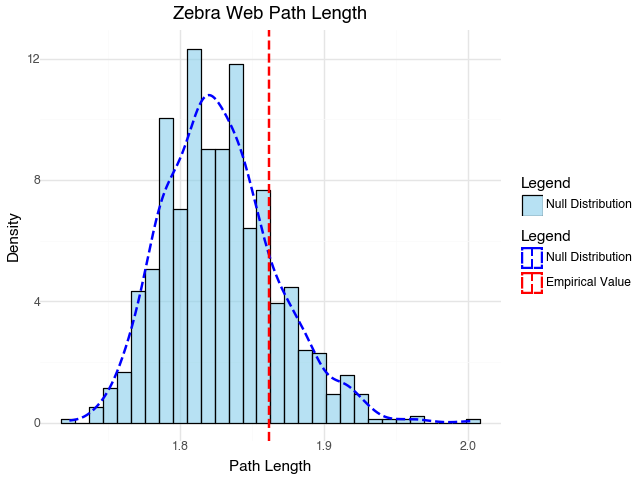
\includegraphics[width=\textwidth]{../figures/zebra_path.png}
        % \caption{Maayan Foodweb Network}
        \label{fig:zebra_network_pathlength}
    \end{minipage}
    \caption{Zebra's Social Network. The left figure shows the clustering coefficient of the network, and the right figure shows the average path length of the network. Histograms of the null distributions of the configuration model are shown in blue, while the empirical values are shown in red.}
    \label{fig:zebra_network}
\end{figure}

The empirical value for the clustering coefficient is larger than the null distribution, while the average pathlength empirical value falls in the null distribution while being greater than mean of the null distribution. This suggests that the network has a higher clustering coefficient than expected by chance, while the average path length is typical of a random network. This implies that the network has a high degree of local clustering, but the average path length is not significantly different from a random network. This suggests that the network is a small-world network, where the average path length is small, but the clustering coefficient is high. This could be due to the network being a social network, where individuals tend to form cliques, but there are short paths between individuals in different cliques.


\subsection*{Biological Network -- Maayan Foodweb}

\begin{figure}[h]
    \centering
    \begin{minipage}{0.45\textwidth}
        \centering
        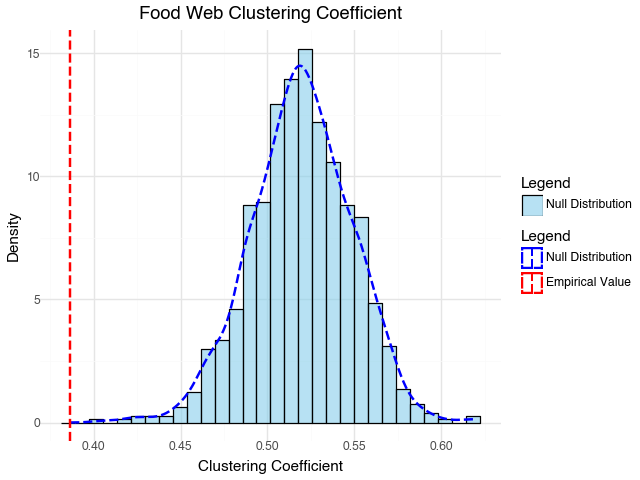
\includegraphics[width=\textwidth]{../figures/food_clustering.png}
        % \caption{Moreno Zebra's Social Network}
        \label{fig:food_network_clustering}
    \end{minipage}
    \hfill
    \begin{minipage}{0.45\textwidth}
        \centering
        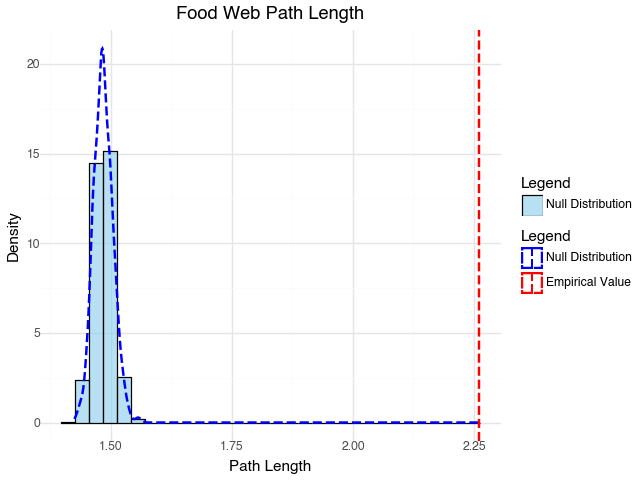
\includegraphics[width=\textwidth]{../figures/food_path.png}
        % \caption{Maayan Foodweb Network}
        \label{fig:food_network_pathlength}
    \end{minipage}
    \caption{Maayan Foodweb. The left figure shows the clustering coefficient of the network, and the right figure shows the average path length of the network. Histograms of the null distributions of the configuration model are shown in blue, while the empirical values are shown in red.}
    \label{fig:foodweb_network}
\end{figure}

The clustering coefficient is lower than the null distribution, while the average path length is larger than the null distribution. This suggests that the network has a lower clustering coefficient than expected by chance, while the average path length is larger than expected by chance. This implies that the network has a low degree of local clustering, and the average path length is larger than expected by chance. This suggests that the network is not a random network, where the average path length is large, and the clustering coefficient is small. This could be due to the network being a food web, where species are not necessarily connected to their neighbors, and there are long paths between species.


\subsection*{Biological Network -- Rhesus Brain Connectome}

\begin{figure}[h]
    \centering
    \begin{minipage}{0.45\textwidth}
        \centering
        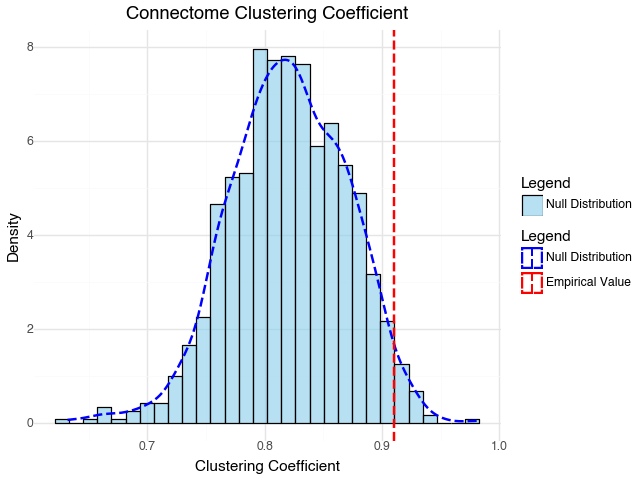
\includegraphics[width=\textwidth]{../figures/connectome_clustering.png}
        % \caption{Moreno Zebra's Social Network}
        \label{fig:connectome_network_clustering}
    \end{minipage}
    \hfill
    \begin{minipage}{0.45\textwidth}
        \centering
        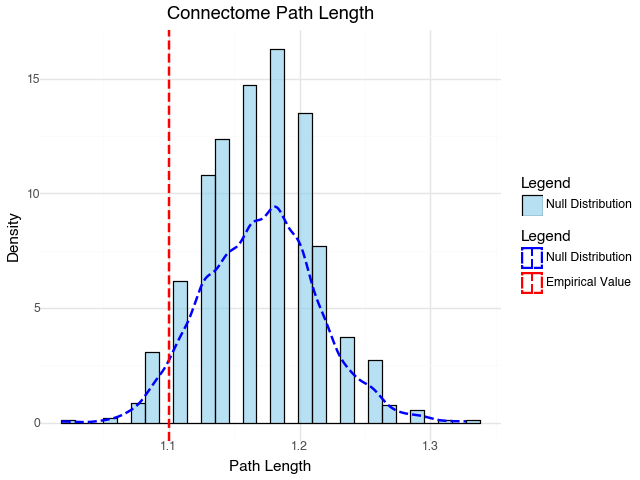
\includegraphics[width=\textwidth]{../figures/connectome_path.png}
        % \caption{Maayan Foodweb Network}
        \label{fig:connectome_network_pathlength}
    \end{minipage}
    \caption{Rhesus Brain Connectome Network. The left figure shows the clustering coefficient of the network, and the right figure shows the average path length of the network. Histograms of the null distributions of the configuration model are shown in blue, while the empirical values are shown in red.}
    \label{fig:Rhesus_connectome_network}
\end{figure}

The clustering coefficient is larger than the mean of the null distribution but not enough to reject the null, while the average path length is smaller than the mean of the null distribution but again not enough to reject the null distribution. This suggests that the network has a higher clustering coefficient than expected by chance, while the average path length is smaller than expected by chance. This implies that the network has a high degree of local clustering, and the average path length is smaller than expected by chance. This suggests that the network is a small-world network, where the average path length is small, but the clustering coefficient is high. This could be due to the network being a brain connectome, where regions of the brain are highly connected, but there are short paths between regions of the brain.

\section*{Problem 5}
\subsection*{Part A}

\begin{figure}[h]
    \centering
    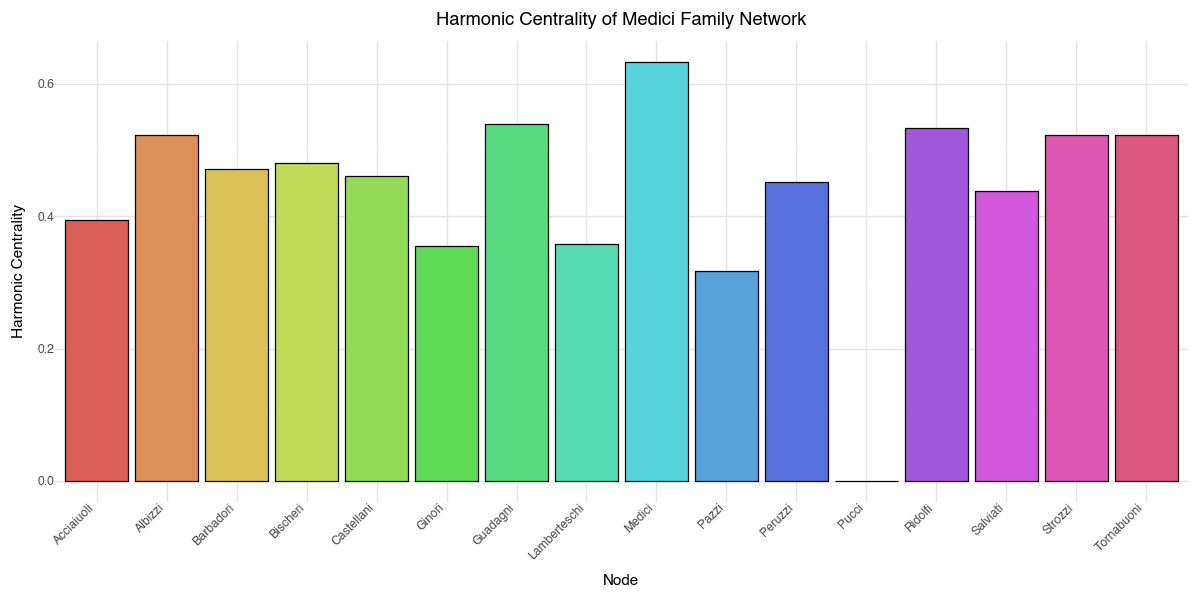
\includegraphics[width=0.8\textwidth]{../figures/harmonic_centrality.png}
    \caption{Harmonic Centrality of the Medici Network.}
    \label{fig:harmonic_centrality}
\end{figure}

The harmonic centralities for each node (or family members of the Medici Family) are shown in Figure \ref{fig:harmonic_centrality}. The highest harmonic centrality appears with Medici and lowest with Pazzi, excluding the Pucci family. The harmonic centrality of the Medici family is higher than the other families in the network, which suggests that the Medici family is more central in the network. This is consistent with the network explanation of the Medici's power, as the Medici family was able to leverage their central position in the network to gain power and influence. The second most important family is the Guadagni family, which has the second highest harmonic centrality in the network. This suggests that the Guadagni family is also central in the network, but not as central as the Medici family.

\subsection*{Part B}

\begin{figure}[h]
    \centering
    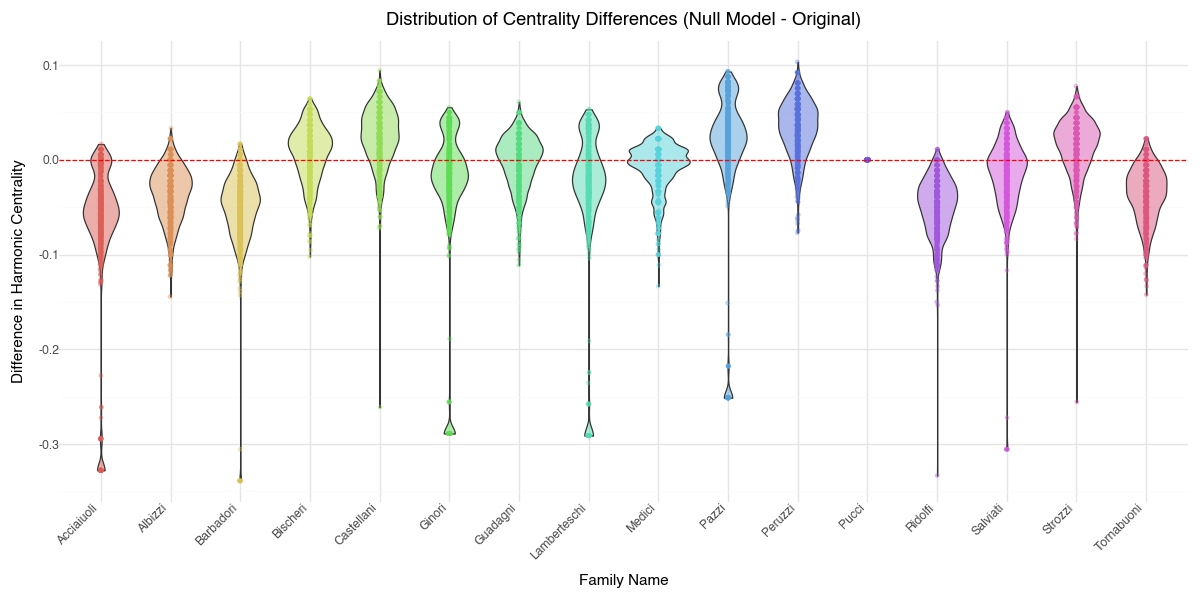
\includegraphics[width=0.8\textwidth]{../figures/centrality_differences.png}
    \caption{Difference in Harmonic Centrality between Data and Null Model.}
    \label{fig:harmonic_centrality_differences}
\end{figure}

The results of the numerical experiment reveal that not all families' harmonic centrality can be explained purely by the network’s degree sequence as shown in Figure \ref{fig:harmonic_centrality_differences}. Families such as the Pazzi, Barbadori, and Ginori have centrality values that are significantly higher than expected under the null model, indicating that their importance within the network is not solely due to their number of connections but also their strategic positioning. In contrast, the Acciaiuoli and Peruzzi families have centrality values that closely align with the null distribution, suggesting that their influence can be explained entirely by degree alone, without additional structural advantages. Most notably, the Medici family's centrality is significantly higher than what would be expected under the null model, demonstrating that their power was not simply a function of how many connections they had, but rather how they positioned themselves within the network. 

\subsection*{Part C}

In the stub-matching null model, the Pucci, Pazzi, and Castellani families have harmonic centrality values explained purely by chance, while the Guadagni, Medici, and Peruzzi families exhibit structural importance beyond what is expected from degree alone (Fig \ref{fig:harmonic_centrality_differences_stub_matching}). Compared to the previous null model, which better preserved the original network’s structure, this model introduces additional randomness, leading to slight differences in which families appear to have centrality driven by factors beyond degree sequence.

\begin{figure}[h]
    \centering
    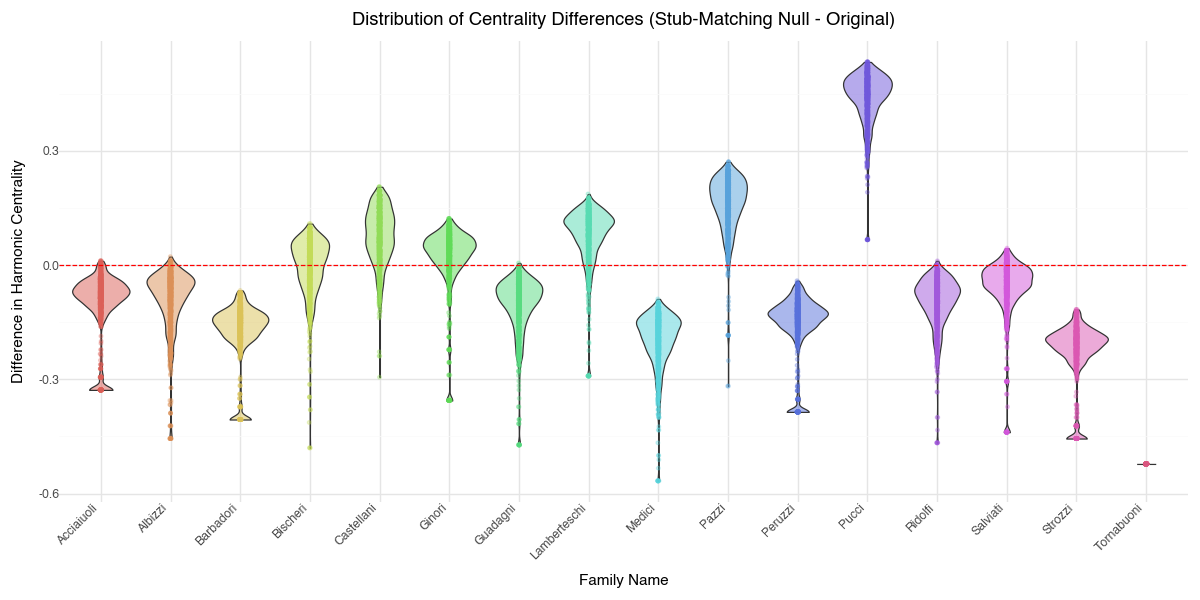
\includegraphics[width=0.8\textwidth]{../figures/centrality_differences_stub_matching.png}
    \caption{Difference in Harmonic Centrality between Data and Null Model with Stub Matching.}
    \label{fig:harmonic_centrality_differences_stub_matching}
\end{figure}

\section*{Problem 6}

\begin{figure}[h]
    \centering
    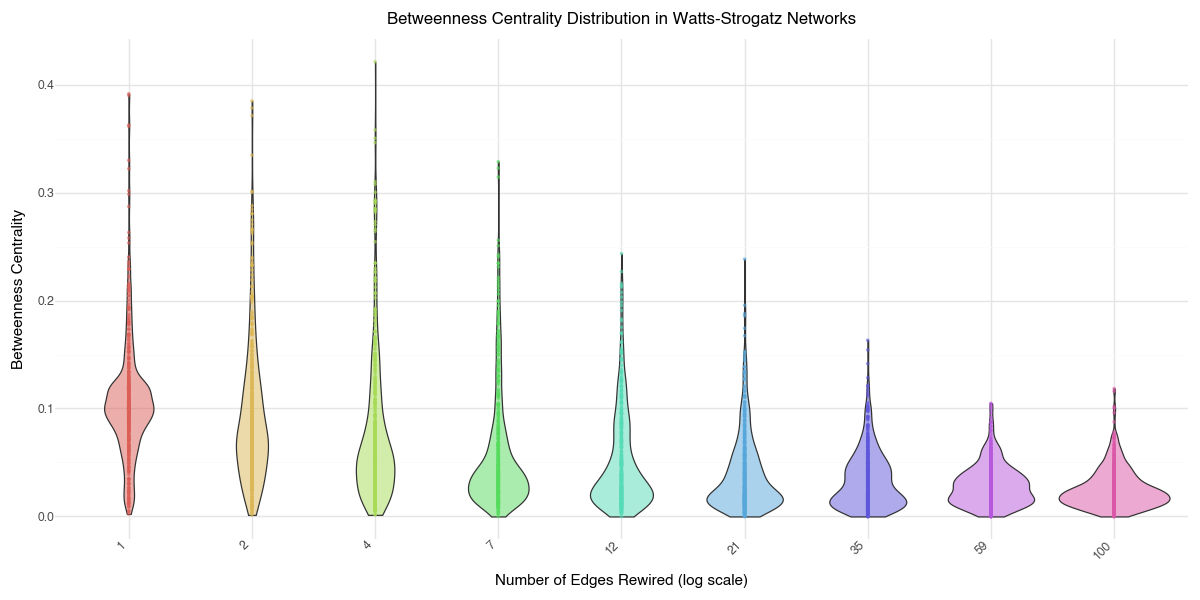
\includegraphics[width=0.8\textwidth]{../figures/betweenness_distribution.png}
    \caption{Betweenness Centrality Distribution in the Watts-Strogratz Networks with different rewiring probabilities.}
    \label{fig:betweenness_distribution}
\end{figure}

See figure \ref{fig:betweenness_distribution}

\section*{Problem 7}

I read the paper ``Predicting poverty and wealth from mobile phone metadata'' by Blumenstock et al. (2016).  The research question they wanted to answer was whether mobile phone metadata could be used to predict an individuals socioeconomic status. They used two main types of datasets from Rwanda's mobile network phone records of its users, and survey data from a subset of this population. The approach they took was to use the datasets and build a machine learning model to predict socioeconomic status. They extracted features from the mobile phone metadata, such as the number of calls and texts made, the number of unique contacts, etc. They then trained and tested their model using the survey data as ground truth.

The authors did a good job of leveraging a large and unique dataset to address their research question.  However, they could have improved their work by discussing potential biases in their dataset more thoroughly. For example, they could have explored how the exclusion of individuals without mobile phones might affect their findings. Additionally they had a limited geographic scope, since they only tested in Rwanda, which could limit the generalizability of their results.

One possible extension of this work could be to apply similar techniques to predict other social outcomes, such as health status or educational attainment. Additionally, future research could investigate the use of mobile phone metadata in different geographic regions to see if the findings are consistent across different contexts. I also think they should expland the geographicical scope of their study to see if their results are generalizable to other regions.

% \section*{Code}

% The code for this assignment can be found at the following GitHub repository: 
% \href{https://github.com/caterer-z-t/CSCI_5352}{https://github.com/caterer-z-t/CSCI_5352}


\end{document}